\ifthenelse{\equal{\doclanguage}{English}}
{\chapter{State of the Art}}
{\chapter{Stato dell'arte}}
\label{sec:sota}

\section{Il modello Property Graph}
Il \textbf{Property Graph}, noto anche come \textit{Labeled Property Graph} (LPG), è un modello di dati emerso nei primi anni 2000 per rappresentare reti di entità interconnesse in modo naturale ed efficiente. Un property graph è un multigrafo orientato in cui i vertici rappresentano entità del dominio applicativo e gli archi rappresentano le relazioni tra esse. A differenza del modello relazionale, in cui le associazioni tra entità sono codificate implicitamente tramite chiavi esterne, nel modello a grafo le relazioni esistono come strutture autonome, tipate e arricchibili con proprietà, rendendo la loro navigazione un'operazione nativa e non derivata.

Il modello si compone strutturalmente di due elementi fondamentali:
\begin{itemize}
\item I \textbf{nodi} (o vertici): rappresentano le entità. Sono caratterizzati da un identificatore univoco, un insieme di \textit{label} che ne classificano la natura semantica e una collezione di proprietà espresse come coppie chiave-valore. Le label consentono di raggruppare i nodi in insiemi omogenei e possono essere modificate dinamicamente senza alterare lo schema del grafo. La possibilità di assegnare zero o più label simultaneamente permette di modellare entità appartenenti a categorie multiple, senza ricorrere a tabelle di associazione aggiuntive.
\item Gli \textbf{archi} (o relazioni): descrivono le connessioni tra i nodi. Ogni arco possiede un identificatore univoco, un nodo sorgente e un nodo destinazione, un'etichetta che ne definisce il tipo semantico e un'eventuale collezione di proprietà. A differenza dei nodi, ogni arco deve avere un tipo e una direzione esplicita, sebbene quest'ultima possa essere ignorata dal motore di calcolo durante le query che richiedono un attraversamento non orientato.
\end{itemize}

Questa flessibilità strutturale si adatta perfettamente alla modellazione di domini complessi. Nel contesto biomedico, ad esempio, consente di rappresentare in modo diretto l'interazione tra un composto chimico (nodo con label \textit{Chemical}) e una patologia (nodo con label \textit{Disease}) attraverso un arco tipato (es. \textit{relates\_to}), potendo inoltre memorizzare all'interno dell'arco stesso le proprietà specifiche di quella interazione, come il peso statistico o la fonte bibliografica della scoperta.

\begin{figure}[ht]
\centering
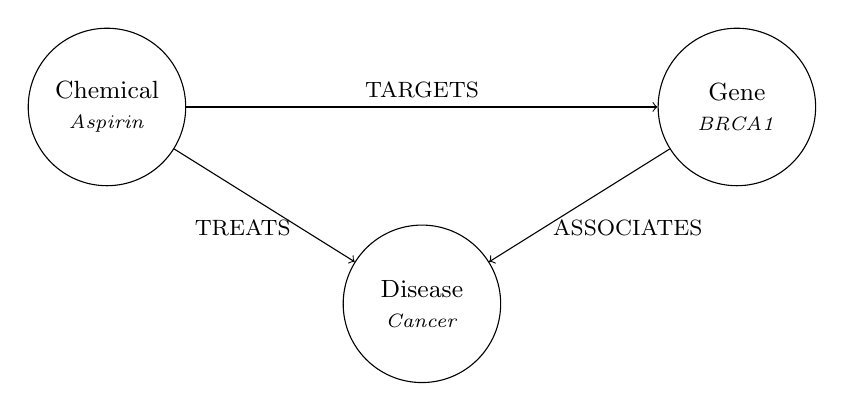
\begin{tikzpicture}[
  node/.style={circle, rounded corners, draw, minimum width=2cm, minimum height=1.5cm, font=\small, align=center},
  every edge/.style={draw, ->, thick},
  prop/.style={font=\footnotesize}
]
  \node[node] (chemical) at (0,0) {Chemical\\\textit{\scriptsize{Aspirin}}};
  \node[node] (gene) at (8,0) {Gene\\\textit{\scriptsize{BRCA1}}};
  \node[node] (disease) at (4,-2.5) {Disease\\\textit{\scriptsize{Cancer}}};

  \draw[->] (chemical) -- node[above, prop] {TARGETS} (gene);
  \draw[->] (gene) -- node[pos=0.7, right, prop] {ASSOCIATES} (disease);
  \draw[->] (chemical) -- node[pos=0.7, left, prop] {TREATS} (disease);
\end{tikzpicture}
\caption{Esempio di Property Graph con nodi etichettati e proprietà}
\label{fig:property_graph_example}
\end{figure}

Il vantaggio computazionale più rilevante del modello LPG rispetto ai sistemi relazionali emerge nelle query di attraversamento (\textit{graph traversal}). In un RDBMS, la navigazione tra entità correlate richiede operazioni di \textit{JOIN} la cui complessità cresce in modo superlineare con la profondità della query e la cardinalità delle tabelle coinvolte. In un database a grafo nativo, ogni passo di traversata ha un costo costante: dato un nodo, l'accesso ai suoi vicini diretti avviene tramite puntatori fisici senza consultare strutture di indice globali, rendendo il modello LPG particolarmente adatto alla bioinformatica.


\section{Neo4j Enterprise e GDS}

Neo4j è un database a grafo \textbf{nativo}, il che significa che implementa il modello a grafo fino al livello di memorizzazione fisica. A differenza dei sistemi che emulano un grafo sopra una tecnologia preesistente, i dati in Neo4j vengono memorizzati esattamente nel modo in cui vengono modellati, senza strati di astrazione intermedi.

Il meccanismo architetturale che rende possibile questa efficienza è l'\textbf{index-free adjacency}: ogni nodo memorizza fisicamente i puntatori diretti agli archi incidenti, i quali a loro volta contengono riferimenti immediati ai nodi sorgente e destinazione. Attraversare una relazione non richiede quindi la consultazione di strutture di indice globali, rendendo il costo di ogni singolo passo di traversata $O(1)$ rispetto alla dimensione complessiva del grafo.

Il linguaggio di interrogazione nativo di Neo4j è \textbf{Cypher}, un linguaggio dichiarativo ottimizzato per i grafi, concettualmente simile a SQL ma progettato per esprimere pattern strutturali e query di attraversamento in modo intuitivo. Cypher è anche alla base del progetto \textit{openCypher} e ha contribuito alla definizione dello standard \textbf{GQL} (\textit{Graph Query Language}).

Per l'analisi algoritmica su larga scala, Neo4j mette a disposizione la libreria \textbf{Graph Data Science} (GDS), un'estensione che fornisce implementazioni parallele di algoritmi su grafi esposti come procedure Cypher. La libreria introduce il concetto di \textbf{graph projection}: prima dell'esecuzione di un algoritmo, il sottografo di interesse viene proiettato in una struttura in memoria separata, denominata \textit{graph catalog}, ottimizzata per il calcolo analitico. Questo meccanismo disaccoppia il layer transazionale da quello analitico, consentendo l'esecuzione di algoritmi massivamente paralleli senza interferire con le operazioni correnti sul database.

\begin{figure}[ht!]
    \centering
    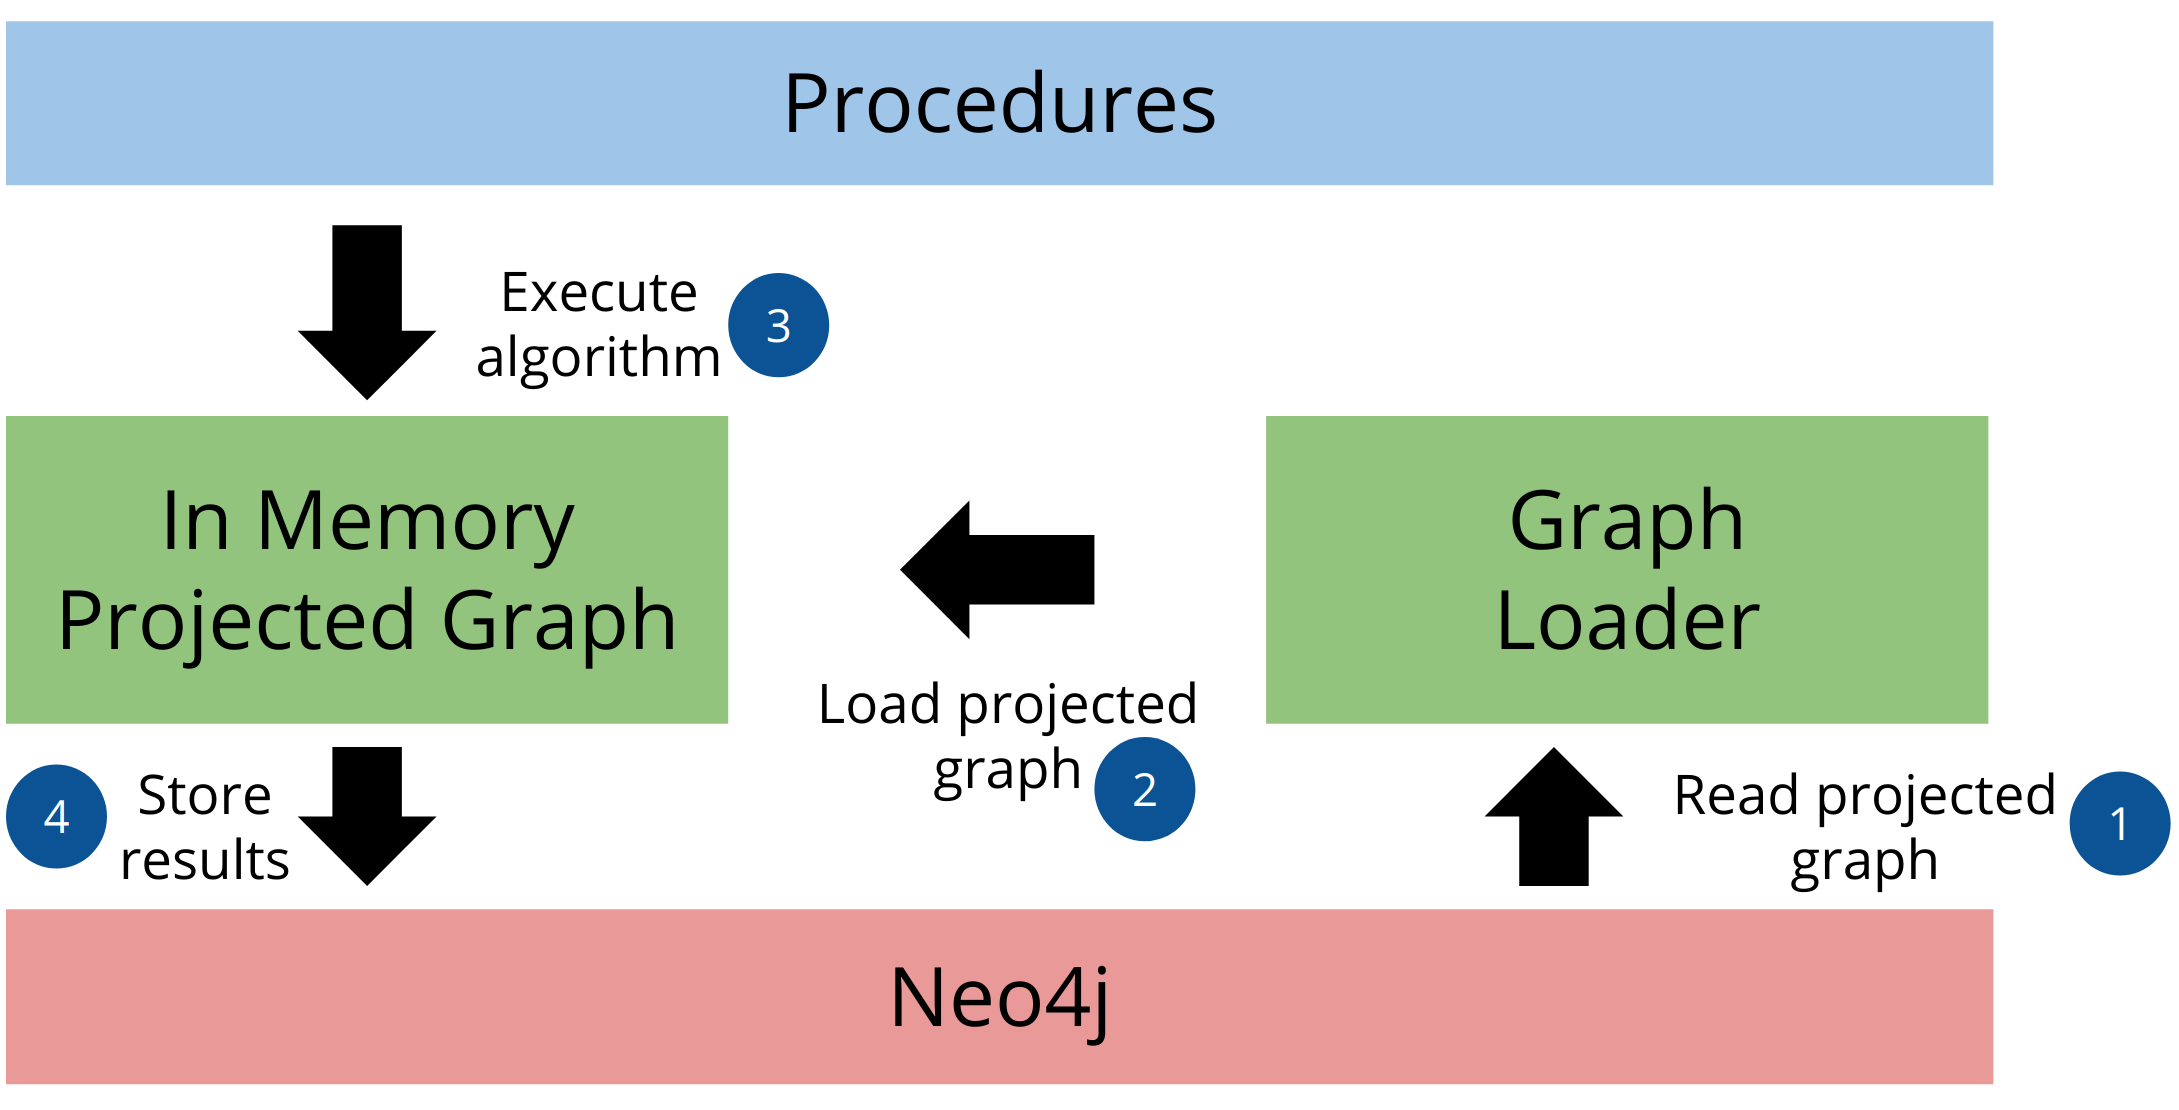
\includegraphics[width=0.75\linewidth]{figures/graph-projection.png}
    \caption{Meccanismo di funzionamento della libreria GDS in Neo4j.}
    \label{fig:gds_projection}
\end{figure}

In questa tesi, Neo4j Enterprise 2026.04.0 viene utilizzato come layer di storage distribuito per PharMeBiNet V3. Il cluster è composto da quattro nodi, un primary e tre secondary, e la libreria GDS costituisce la base concettuale del meccanismo di estrazione del sottografo verso PyTorch Geometric, descritto nel capitolo dei metodi.


\section{Graph Embeddings e Graph Neural Networks}
I \textbf{graph embedding} sono funzioni che proiettano i nodi di un grafo in uno spazio vettoriale continuo a bassa dimensionalità, preservando proprietà strutturali e semantiche della rete originale. L'obiettivo è trasformare entità discrete — nodi identificati da un ID o da una stringa — in vettori numerici su cui applicare algoritmi di Machine Learning standard.














\begin{figure}[ht!]
\centering
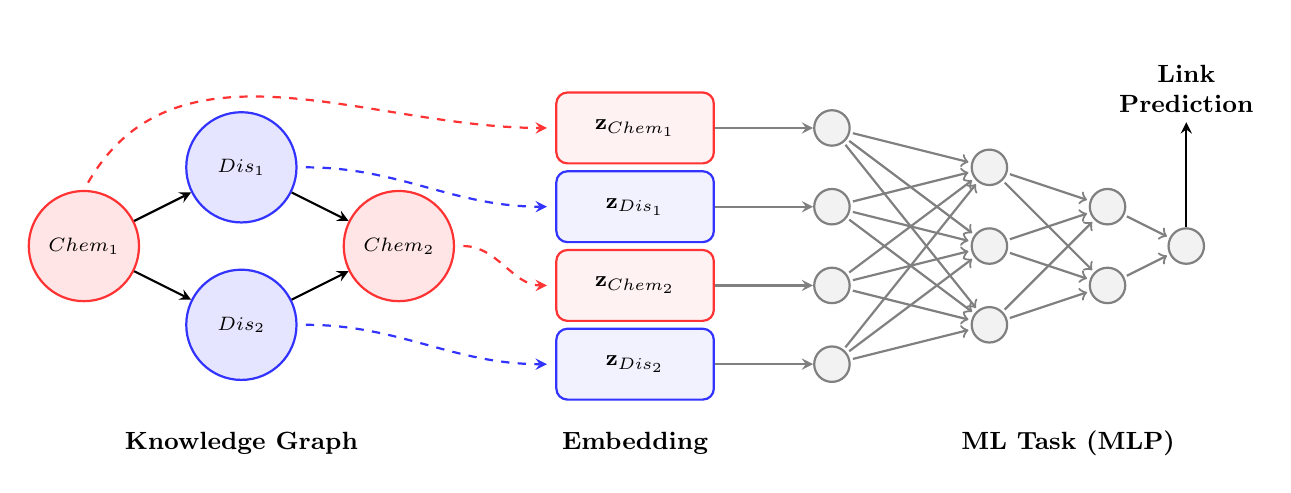
\begin{tikzpicture}[
  node_chem/.style={circle, draw=red!80, fill=red!10, thick, minimum size=1.4cm, font=\scriptsize},
  node_dis/.style={circle, draw=blue!80, fill=blue!10, thick, minimum size=1.4cm, font=\scriptsize},
  vec_chem/.style={rectangle, draw=red!80, fill=red!5, rounded corners, minimum width=2cm, minimum height=0.9cm, font=\footnotesize, align=center, thick},
  vec_dis/.style={rectangle, draw=blue!80, fill=blue!5, rounded corners, minimum width=2cm, minimum height=0.9cm, font=\footnotesize, align=center, thick},
  ml_node/.style={circle, draw=gray, fill=gray!10, thick, minimum size=0.45cm},
  arrow/.style={->, thick, >=stealth},
  map_arrow/.style={->, thick, dashed, >=stealth, shorten <=3pt, shorten >=3pt},
  connect/.style={->, gray, thick, shorten <=1pt, shorten >=1pt}
]

  % KNOWLEDGE GRAPH
  \node[node_chem] (c1) at (0,4)   {$\text{Chem}_1$};
  \node[node_dis]  (d1) at (2,5)   {$\text{Dis}_1$};
  \node[node_dis] (d2) at (2,3)   {$\text{Dis}_2$};
  \node[node_chem]  (c2) at (4,4)   {$\text{Chem}_2$};


  \draw[arrow] (c1) -- (d1);
  \draw[arrow] (c1) -- (d2);
  \draw[arrow] (d1) -- (c2);
  \draw[arrow] (d2) -- (c2);

  \node[font=\bfseries\small] at (2,1.5) {Knowledge Graph};

  % EMBEDDED REPRESENTATIONS
  \node[vec_chem] (v_c1) at (7,5.5) {$\mathbf{z}_{\text{Chem}_1}$};
  \node[vec_dis]  (v_d1) at (7,4.5) {$\mathbf{z}_{\text{Dis}_1}$};
  \node[vec_chem] (v_c2) at (7,3.5) {$\mathbf{z}_{\text{Chem}_2}$};
  \node[vec_dis]  (v_d2) at (7,2.5) {$\mathbf{z}_{\text{Dis}_2}$};

  % Frecce di mappatura curve (senza sovrapposizioni)
  \draw[map_arrow, red!80]  (c1.north) to[out=60, in=180] (v_c1.west);
  \draw[map_arrow, blue!80] (d1.east) to[out=0, in=180] (v_d1.west);
  \draw[map_arrow, red!80]  (c2.east) to[out=0, in=180] (v_c2.west);
  \draw[map_arrow, blue!80] (d2.east) to[out=0, in=180] (v_d2.west);

  \node[font=\bfseries\small] at (7,1.5) {Embedding};

  % MACHINE LEARNING TASK
  % Input layer
  \node[ml_node] (in1) at (9.5,5.5) {};
  \node[ml_node] (in2) at (9.5,4.5) {};
  \node[ml_node] (in3) at (9.5,3.5) {};
  \node[ml_node] (in4) at (9.5,2.5) {};

  % Hidden layer 1
  \node[ml_node] (h1) at (11.5,5) {};
  \node[ml_node] (h2) at (11.5,4) {};
  \node[ml_node] (h3) at (11.5,3) {};

  % Hidden layer 2
  \node[ml_node] (h4) at (13,4.5) {};
  \node[ml_node] (h5) at (13,3.5) {};

  % Output
  \node[ml_node] (out) at (14,4) {};

  % Predizione
  \node[font=\small\bfseries, align=center] (pred) at (14,6) {Link\\Prediction};

  % Connessioni dagli embedding agli input (ortogonali, nessun incrocio)
  \draw[arrow, gray] (v_c1.east) -- ++(0.8,0) |- (in1.west);
  \draw[arrow, gray] (v_d1.east) -- ++(0.8,0) |- (in2.west);
  \draw[arrow, gray] (v_c2.east) -- ++(0.8,0) |- (in3.west);
  \draw[arrow, gray] (v_d2.east) -- ++(0.8,0) |- (in4.west);

  % Connessioni fully‑connected tra gli strati della MLP
  \foreach \i in {in1,in2,in3,in4} {
    \foreach \j in {h1,h2,h3} {
      \draw[connect] (\i) -- (\j);
    }
  }
  \foreach \i in {h1,h2,h3} {
    \foreach \j in {h4,h5} {
      \draw[connect] (\i) -- (\j);
    }
  }
  \foreach \i in {h4,h5} {
    \draw[connect] (\i) -- (out);
  }

  \draw[arrow, thick, >=stealth] (out) -- (pred);

  \node[font=\bfseries\small] at (12.5,1.5) {ML Task (MLP)};

\end{tikzpicture}
\caption{Architettura end-to-end: dal Knowledge Graph eterogeneo (nodi Chemical e Disease) all'estrazione degli embedding nello spazio latente, fino al task di Link Prediction tramite rete neurale (MLP).}
\label{fig:end_to_end_pipeline}
\end{figure}

















































Le \textbf{Graph Neural Networks} (GNN) sono la famiglia di modelli che apprende questi embedding direttamente dalla struttura del grafo, senza richiedere feature ingegnerizzate manualmente. Il meccanismo comune a tutte le GNN è il \textbf{message passing}: per ogni nodo, l'embedding viene aggiornato iterativamente aggregando le rappresentazioni dei nodi vicini. Dopo $k$ iterazioni, l'embedding di un nodo cattura informazioni strutturali fino a $k$ salti di distanza nella rete.

Formalmente, dato un nodo $v$ al layer $l$, l'aggiornamento segue lo schema:

\begin{equation}
\mathbf{h}_v^{(l)} = \text{UPDATE}\left(\mathbf{h}_v^{(l-1)},\ \text{AGGREGATE}\left(\left\{\mathbf{h}_u^{(l-1)} : u \in \mathcal{N}(v)\right\}\right)\right)
\label{eq:message_passing}
\end{equation}

dove $\mathcal{N}(v)$ indica l'insieme dei vicini di $v$, e le funzioni \textsc{Aggregate} e \textsc{Update} variano a seconda dell'architettura specifica.

I tre algoritmi analizzati in questa tesi rappresentano tre approcci distinti a questo problema, differenziandosi per strategia di aggregazione, gestione dell'eterogeneità del grafo e tipo di task per cui sono stati progettati. La tabella \ref{tab:algo_comparison} ne riassume le caratteristiche principali.

\begin{table}[h!]
\centering
\small
\begin{tabular}{llll}
\toprule
\textbf{Algoritmo} & \textbf{Approccio} & \textbf{Eterogeneità} & \textbf{Task ideale} \\
\midrule
GraphSAGE & Aggregazione vicini & Omogeneo & Link prediction, node classification \\
TransE    & Traslazione vettoriale & Relazioni tipizzate & Link prediction su KG \\
HashGNN   & Hashing + proiezione & Eterogeneo nativo & Grafi multi-tipo \\
\bottomrule
\end{tabular}
\caption{Confronto dei tre algoritmi analizzati.}
\label{tab:algo_comparison}
\end{table}


\section{GraphSAGE}

GraphSAGE (\textit{Graph SAmple and aggreGatE}) è un algoritmo di graph embedding induttivo proposto da Hamilton et al. nel 2017. A differenza degli approcci trasduttivi, che calcolano embedding solo per i nodi presenti durante il training, GraphSAGE apprende una \textbf{funzione di aggregazione} generalizzabile a nodi non visti, rendendolo adatto a grafi dinamici e a larga scala.

\subsection{Meccanismo di funzionamento}

L'intuizione alla base di GraphSAGE è semplice: l'identità di un nodo è definita dal suo vicinato. Invece di apprendere un vettore per ogni nodo individualmente, l'algoritmo apprende come aggregare le feature dei vicini per produrre una rappresentazione del nodo stesso.

Il forward pass si articola in due fasi per ogni layer $l$:

\begin{enumerate}
  \item \textbf{Campionamento}: per ogni nodo $v$, viene selezionato un sottoinsieme fisso $\mathcal{S}(v) \subseteq \mathcal{N}(v)$ di vicini. Il campionamento è necessario per controllare il costo computazionale su nodi ad alto grado.
  \item \textbf{Aggregazione}: le rappresentazioni dei vicini campionati vengono aggregate e combinate con la rappresentazione corrente del nodo.
\end{enumerate}

Formalmente:
\begin{equation}
\mathbf{h}_{\mathcal{N}(v)}^{(l)} = \text{AGGREGATE}_l\left(\left\{\mathbf{h}_u^{(l-1)} : u \in \mathcal{S}(v)\right\}\right)
\end{equation}
\begin{equation}
\mathbf{h}_v^{(l)} = \sigma\left(\mathbf{W}^{(l)} \cdot \left[\mathbf{h}_v^{(l-1)} \,\|\, \mathbf{h}_{\mathcal{N}(v)}^{(l)}\right]\right)
\end{equation}

dove $\|$ indica la concatenazione, $\mathbf{W}^{(l)}$ è la matrice di pesi apprendibile al layer $l$ e $\sigma$ è una funzione di attivazione non lineare. Gli aggregatori supportati includono \textit{Mean} (media delle rappresentazioni dei vicini), \textit{Pool} (max-pooling dopo una trasformazione lineare) e \textit{LSTM} (aggregazione sequenziale su una permutazione casuale dei vicini).

\begin{figure}[ht]
\centering
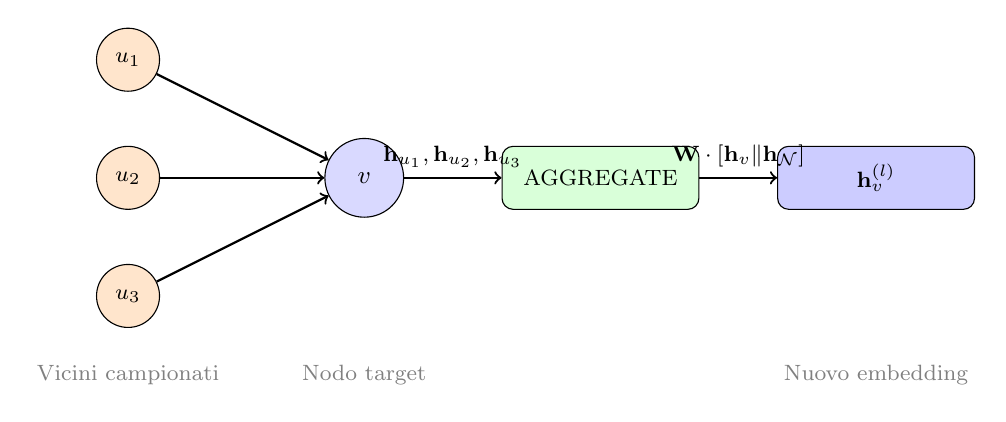
\begin{tikzpicture}[
  mainnode/.style={circle, draw, fill=blue!15, minimum size=1cm, font=\small},
  neighnode/.style={circle, draw, fill=orange!20, minimum size=0.8cm, font=\footnotesize},
  aggbox/.style={rectangle, draw, rounded corners, fill=green!15,
                 minimum width=2.5cm, minimum height=0.8cm, font=\footnotesize},
  outbox/.style={rectangle, draw, rounded corners, fill=blue!20,
                 minimum width=2.5cm, minimum height=0.8cm, font=\footnotesize},
  arrow/.style={->, thick}
]
  \node[neighnode] (n1) at (-3, 1.5)  {$u_1$};
  \node[neighnode] (n2) at (-3, 0)    {$u_2$};
  \node[neighnode] (n3) at (-3, -1.5) {$u_3$};
  \node[mainnode]  (v)  at (0, 0)     {$v$};

  \draw[arrow] (n1) -- (v);
  \draw[arrow] (n2) -- (v);
  \draw[arrow] (n3) -- (v);

  \node[aggbox] (agg) at (3, 0) {AGGREGATE};
  \draw[arrow] (v) -- node[above, font=\footnotesize]{$\mathbf{h}_{u_1}, \mathbf{h}_{u_2}, \mathbf{h}_{u_3}$} (agg);

  \node[outbox] (out) at (6.5, 0) {$\mathbf{h}_v^{(l)}$};
  \draw[arrow] (agg) -- node[above, font=\footnotesize]{$\mathbf{W} \cdot [\mathbf{h}_v \| \mathbf{h}_\mathcal{N}]$} (out);

  \node[font=\footnotesize, gray] at (-3, -2.5) {Vicini campionati};
  \node[font=\footnotesize, gray] at (0, -2.5)  {Nodo target};
  \node[font=\footnotesize, gray] at (6.5, -2.5) {Nuovo embedding};
\end{tikzpicture}
\caption{Il meccanismo di aggregazione di GraphSAGE: i vicini campionati vengono aggregati e combinati con la rappresentazione del nodo target.}
\label{fig:graphsage_aggregation}
\end{figure}

\subsection{Pipeline per la link prediction}

Nel contesto di questa tesi, GraphSAGE viene impiegato per il task di link prediction tra nodi \textit{Chemical} e \textit{Disease}. La pipeline si articola in tre componenti distinti.

\begin{figure}[ht]
\centering
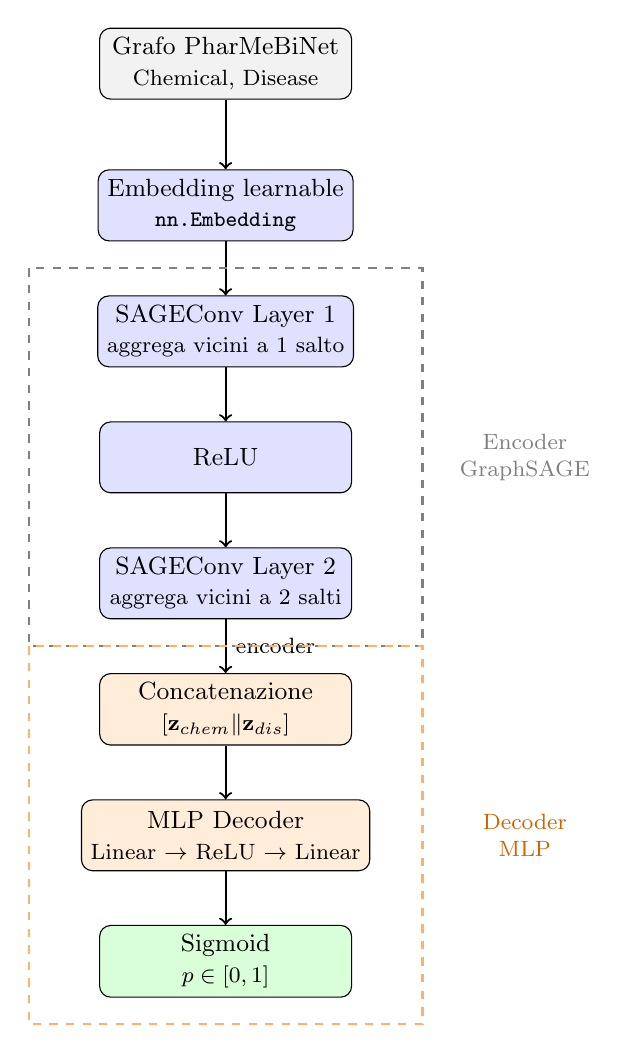
\begin{tikzpicture}[
  box/.style={rectangle, draw, rounded corners, minimum width=3.2cm,
              minimum height=0.9cm, font=\small, align=center},
  encoder/.style={box, fill=blue!12},
  decoder/.style={box, fill=orange!15},
  input/.style={box, fill=gray!10},
  output/.style={box, fill=green!15},
  arrow/.style={->, thick}
]
  \node[input]   (graph)   at (0, 6)    {Grafo PharMeBiNet\\{\footnotesize Chemical, Disease}};
  \node[encoder] (emb)     at (0, 4.2)  {Embedding learnable\\{\footnotesize \texttt{nn.Embedding}}};
  \node[encoder] (conv1)   at (0, 2.6)  {SAGEConv Layer 1\\{\footnotesize aggrega vicini a 1 salto}};
  \node[encoder] (relu)    at (0, 1.0)  {ReLU};
  \node[encoder] (conv2)   at (0, -0.6) {SAGEConv Layer 2\\{\footnotesize aggrega vicini a 2 salti}};
  \node[decoder] (concat)  at (0, -2.2) {Concatenazione\\{\footnotesize $[\mathbf{z}_{chem} \| \mathbf{z}_{dis}]$}};
  \node[decoder] (mlp)     at (0, -3.8) {MLP Decoder\\{\footnotesize Linear $\to$ ReLU $\to$ Linear}};
  \node[output]  (sigmoid) at (0, -5.4) {Sigmoid\\{\footnotesize $p \in [0, 1]$}};

  \draw[arrow] (graph)   -- (emb);
  \draw[arrow] (emb)     -- (conv1);
  \draw[arrow] (conv1)   -- (relu);
  \draw[arrow] (relu)    -- (conv2);
  \draw[arrow] (conv2)   -- node[right, font=\footnotesize]{encoder} (concat);
  \draw[arrow] (concat)  -- (mlp);
  \draw[arrow] (mlp)     -- (sigmoid);

  \draw[dashed, thick, gray] 
    (-2.5, 3.4) rectangle (2.5, -1.4);
  \node[gray, font=\footnotesize, align=center] at (3.8, 1.0) {Encoder\\GraphSAGE};

  \draw[dashed, thick, orange!60]
    (-2.5, -1.4) rectangle (2.5, -6.2);
  \node[orange!80!black, font=\footnotesize, align=center] at (3.8, -3.8) {Decoder\\MLP};

\end{tikzpicture}
\caption{Pipeline completa di GraphSAGE per la link prediction Chemical→Disease.}
\label{fig:graphsage_pipeline}
\end{figure}

\textbf{Encoder}: poiché i nodi Chemical e Disease in PharMeBiNet non possiedono feature numeriche — sono identificati solo da stringhe come \texttt{DB00620} o \texttt{MONDO:0000004} — le feature iniziali sono embedding learnable, una tabella di vettori inizializzati casualmente e ottimizzati durante il training. Gli embedding di Chemical e Disease vengono fusi in un unico tensore omogeneo tramite concatenazione, e gli indici Disease vengono traslati di \texttt{num\_chemical} posizioni per evitare collisioni. Due layer SAGEConv propagano l'informazione strutturale del vicinato.

\textbf{Decoder}: dati gli embedding $\mathbf{z}_{chem}$ e $\mathbf{z}_{dis}$ di una coppia di nodi, il decoder li concatena e li passa attraverso un MLP (\textit{Multi-Layer Perceptron}) con attivazione finale sigmoid, producendo uno score $p \in [0, 1]$ che rappresenta la probabilità che il link esista.

\textbf{Training}: il modello viene addestrato su link positivi (archi reali) e link negativi generati casualmente, minimizzando la \textit{binary cross-entropy loss}. Il 10\% degli archi viene tenuto nascosto per la valutazione finale tramite \texttt{RandomLinkSplit}.

\subsection{Vantaggi e limitazioni}

GraphSAGE è induttivo, scalabile e converge rapidamente. Il suo principale limite su PharMeBiNet è che tratta il grafo come omogeneo: non distingue i 410 tipi di relazione presenti nel dataset, aggregando indiscriminatamente vicini di tipo diverso. Su nodi ad alto grado come le proteine (grado medio 232), il campionamento fisso introduce rumore informativo perdendo parte del contesto biologico.


\section{TransE}

TransE (\textit{Translating Embeddings}) è un modello di knowledge graph embedding proposto da Bordes et al. nel 2013. A differenza delle GNN che aggregano informazioni strutturali dai vicini, TransE apprende embedding per entità e relazioni modellando le relazioni come \textbf{traslazioni nello spazio vettoriale}.

\subsection{Meccanismo di funzionamento}

L'intuizione di TransE è geometrica: data una tripla valida $(h, r, t)$ — dove $h$ è il nodo testa, $r$ la relazione e $t$ il nodo coda — il modello ottimizza gli embedding affinché $\mathbf{h} + \mathbf{r} \approx \mathbf{t}$.

\begin{figure}[ht]
\centering
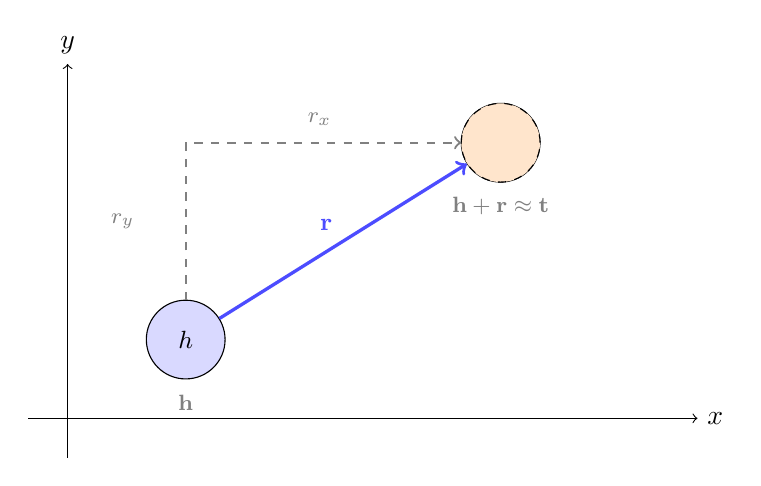
\begin{tikzpicture}[
  arrow/.style={->, thick},
  node/.style={circle, draw, fill=blue!15, minimum size=1cm, font=\small}
]
  \draw[->] (-0.5,0) -- (8,0) node[right] {$x$};
  \draw[->] (0,-0.5) -- (0,4.5) node[above] {$y$};

  \node[node] (h) at (1.5, 1.0) {$h$};
  \node[node] (t) at (5.5, 3.5) {$t$};

  \draw[arrow, blue!70, very thick] (h) -- 
    node[above left, font=\small]{$\mathbf{r}$} (t);

  \node[circle, draw, dashed, fill=orange!20, minimum size=1cm, font=\small] 
    (hpr) at (5.5, 3.5) {};

  \node[font=\footnotesize, gray] at (1.5, 0.2) {$\mathbf{h}$};
  \node[font=\footnotesize, gray] at (5.5, 2.7) {$\mathbf{h} + \mathbf{r} \approx \mathbf{t}$};

  \draw[arrow, dashed, gray] (1.5, 1.5) -- (1.5, 3.5) -- (5.0, 3.5);
  \node[font=\footnotesize, gray] at (0.7, 2.5) {$r_y$};
  \node[font=\footnotesize, gray] at (3.2, 3.8) {$r_x$};
\end{tikzpicture}
\caption{L'intuizione geometrica di TransE: la relazione $\mathbf{r}$ è un vettore di traslazione da $\mathbf{h}$ a $\mathbf{t}$ nello spazio degli embedding.}
\label{fig:transe_geometry}
\end{figure}

La funzione di scoring per una tripla $(h, r, t)$ è la distanza L2 tra $\mathbf{h} + \mathbf{r}$ e $\mathbf{t}$:

\begin{equation}
f(h, r, t) = \|\mathbf{h} + \mathbf{r} - \mathbf{t}\|_2
\end{equation}

Un valore basso indica una tripla plausibile, un valore alto indica una tripla falsa. Il training usa una \textbf{margin ranking loss}:

\begin{equation}
\mathcal{L} = \sum_{(h,r,t) \in S} \sum_{(h',r,t') \in S'} \max\left(0,\ \gamma + f(h,r,t) - f(h',r,t')\right)
\end{equation}

dove $S$ è l'insieme delle triple positive, $S'$ quello delle triple negative generate per corruzione, e $\gamma$ è il margine. La loss penalizza i casi in cui il punteggio della tripla negativa non supera quello della tripla positiva di almeno $\gamma$.

\subsection{Vantaggi e limitazioni}

TransE è computazionalmente efficiente e cattura esplicitamente la semantica delle relazioni tramite il vettore $\mathbf{r}$, il che lo rende particolarmente adatto a knowledge graph con molti tipi di relazione come PharMeBiNet. Il suo principale limite è che è un modello \textbf{trasduttivo}: non generalizza a nodi non visti durante il training. Presenta inoltre difficoltà nel modellare relazioni simmetriche ($h \to t$ e $t \to h$ dello stesso tipo) poiché la traslazione è direzionale per definizione.


\section{HashGNN}

HashGNN è un algoritmo di graph embedding progettato nativamente per grafi eterogenei, proposto da Ni et al e successivamente integrato nella libreria Neo4j GDS. A differenza di GraphSAGE, che fonde i diversi tipi di nodo in un unico spazio omogeneo, HashGNN mantiene \textbf{spazi di rappresentazione separati} per ogni tipo di nodo, usando funzioni di hashing casuali per arricchire le feature senza aumentare il numero di parametri apprendibili.

\subsection{Meccanismo di funzionamento}

L'idea centrale di HashGNN è sostituire le proiezioni lineari apprendibili con \textbf{proiezioni casuali fisse} ispirate al \textit{Locality-Sensitive Hashing} (LSH). Per ogni nodo, l'embedding viene proiettato attraverso $K$ matrici casuali fisse $\mathbf{R}_1, \dots, \mathbf{R}_K$, e i risultati vengono binarizzati tramite la funzione segno:

\begin{equation}
\mathbf{h}_v^{hash} = \left[\text{sign}(\mathbf{x}_v \mathbf{R}_1^\top) \,\|\, \dots \,\|\, \text{sign}(\mathbf{x}_v \mathbf{R}_K^\top)\right]
\end{equation}

Questo produce $K$ viste diverse dello stesso nodo, catturando aspetti complementari della struttura locale. Le proiezioni fisse non vengono aggiornate durante il training: solo i layer lineari successivi (\textit{projection layers}) sono apprendibili, uno per ogni tipo di nodo.

\begin{figure}[ht]
\centering
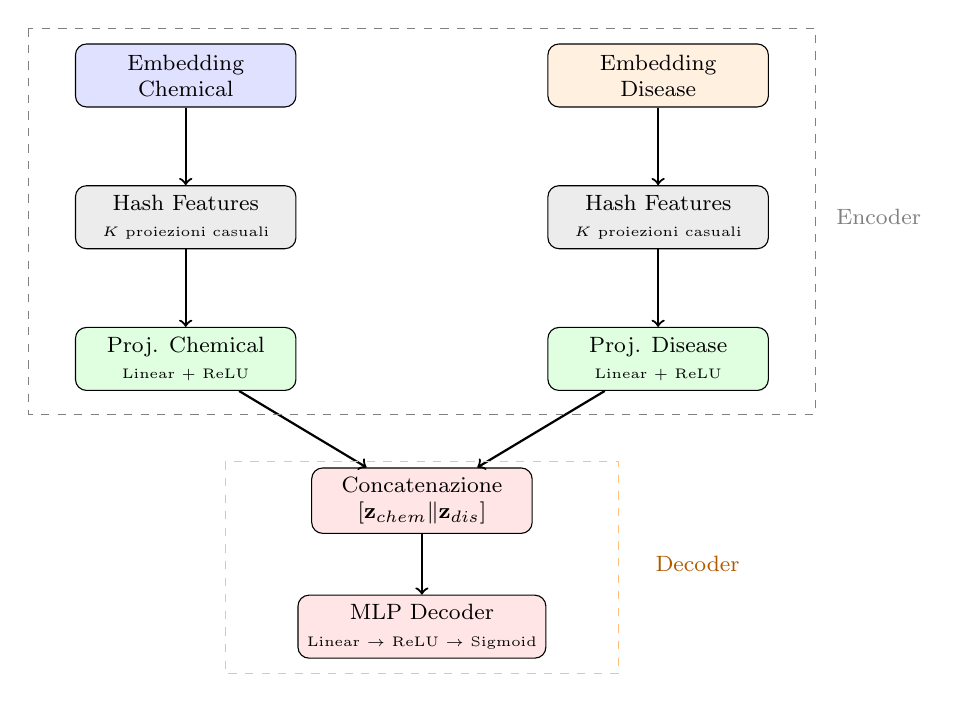
\begin{tikzpicture}[
  box/.style={rectangle, draw, rounded corners, minimum width=2.8cm,
              minimum height=0.8cm, font=\footnotesize, align=center},
  chembox/.style={box, fill=blue!12},
  disbox/.style={box, fill=orange!12},
  hashbox/.style={box, fill=gray!15},
  projbox/.style={box, fill=green!12},
  decbox/.style={box, fill=red!10},
  arrow/.style={->, thick}
]
  \node[chembox] (ce)  at (-3, 4)   {Embedding\\Chemical};
  \node[disbox]  (de)  at (3, 4)    {Embedding\\Disease};

  \node[hashbox] (ch)  at (-3, 2.2) {Hash Features\\{\tiny $K$ proiezioni casuali}};
  \node[hashbox] (dh)  at (3, 2.2)  {Hash Features\\{\tiny $K$ proiezioni casuali}};

  \node[projbox] (cp)  at (-3, 0.4) {Proj. Chemical\\{\tiny Linear + ReLU}};
  \node[projbox] (dp)  at (3, 0.4)  {Proj. Disease\\{\tiny Linear + ReLU}};

  \node[decbox]  (cat) at (0, -1.4) {Concatenazione\\$[\mathbf{z}_{chem} \| \mathbf{z}_{dis}]$};
  \node[decbox]  (mlp) at (0, -3.0) {MLP Decoder\\{\tiny Linear $\to$ ReLU $\to$ Sigmoid}};

  \draw[arrow] (ce)  -- (ch);
  \draw[arrow] (de)  -- (dh);
  \draw[arrow] (ch)  -- (cp);
  \draw[arrow] (dh)  -- (dp);
  \draw[arrow] (cp)  -- (cat);
  \draw[arrow] (dp)  -- (cat);
  \draw[arrow] (cat) -- (mlp);

  \draw[dashed, gray] (-5, 4.6) rectangle (5, -0.3);
  \node[gray, font=\footnotesize] at (5.8, 2.2) {Encoder};

  \draw[dashed, orange!50] (-2.5, -0.9) rectangle (2.5, -3.6);
  \node[orange!70!black, font=\footnotesize] at (3.5, -2.2) {Decoder};

\end{tikzpicture}
\caption{Architettura di HashGNN per la link prediction: Chemical e Disease mantengono spazi di embedding separati fino al decoder.}
\label{fig:hashgnn_architecture}
\end{figure}

\subsection{Vantaggi e limitazioni}

HashGNN gestisce nativamente l'eterogeneità del grafo mantenendo proiezioni distinte per ogni tipo di nodo, il che lo rende teoricamente più adatto di GraphSAGE su dataset come PharMeBiNet. Le proiezioni fisse riducono il numero di parametri apprendibili e il rischio di overfitting. Il principale svantaggio è la \textbf{convergenza più lenta}: i layer lineari devono compensare la casualità delle proiezioni hash, richiedendo un numero maggiore di epoche per stabilizzarsi rispetto a GraphSAGE, che opera con pesi densi direttamente ottimizzabili.